%
\section{\color{red}Introduction\label{ptInt}}

%
\section{Methods \label{meth}}


%
\subsection{Model}

%
The Schnute production function is a three-parameter generalization of many of
the most common two-parameter production functions \cite{deriso_harvesting_1980, schnute_general_1985}. %\shortcit{deriso_harvesting_1980}. 
It can be written in the following form, with parameters $\alpha$, $\beta$, and $\gamma$,
%
\begin{align}
P_s(B; [\alpha, \beta, \gamma]) = \alpha B (1-\beta\gamma B)^{\frac{1}{\gamma}}.
\end{align}

%
\begin{wrapfigure}{r}{0.5\textwidth}
%\begin{figure}[h!]
%\begin{minipage}[h!]{0.64\textwidth}
\vspace{-0.6cm}
%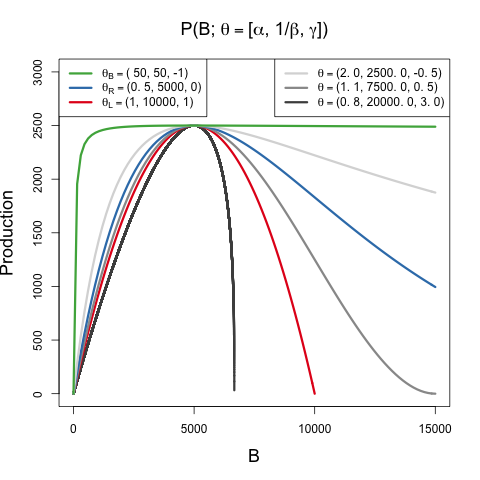
\includegraphics[width=0.5\textwidth]{plots/derisoSrr.png}
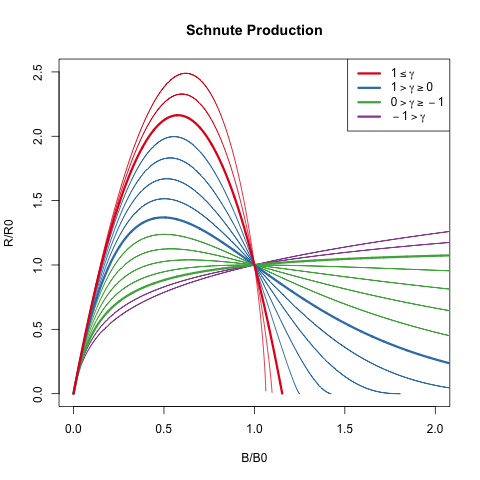
\includegraphics[width=0.49\textwidth]{../gpBias/g3.png}
\vspace{-1cm}
%\end{minipage}
%\begin{minipage}[h!]{0.3\textwidth}
\caption{
%\onehalfspacing
The Schnute production function plotted across a variety of parameter
values. Regimes of similarly behaving curves are grouped by color.
% BH-like, Ricker-like, and Logistic production are shown in
%green, blue, and red respectively.
}
\label{sRegimes}
%\end{minipage}
\end{wrapfigure}
%\end{figure}

%
The BH and Logistic production functions arise when $\gamma$ is fixed to -1 or
1 respectively. The Ricker model is a limiting case as $\gamma\rightarrow0$. %\shortcite{schnute_general_1985}.
For $\gamma<-1$ a family of strictly increasing Cushing-like curves arise,
culminating in linear production as $\gamma\to-\infty$. These special cases form
natural regimes of similarly behaving production functions as seen in Figure (\ref{sRegimes}).

%
The behavior of RP inference under the BH model is of particular interest due
to the overwhelming popularity of the BH assumption in fisheries models.
%% 
%Inference of BH productivity parameters under a wide variety of data is of particular 
%interest due to the overwhelming popularity of the BH assumption in fisheries 
%models. 
Since Schnute production models can represent a quantifiably wide variety
of possible productivity behaviors, they present an ideal simulation
environment for inquiry of the reliability of inference under the BH
assumption.


%
Under Schnute production, biomass dynamics evolve according to the following ODE,
%
\begin{align}
\frac{dB}{dt} = P_s(B;\theta) - (M+F)B. \label{schnuteSimple}
\end{align}
%
This equation largely takes the same form as previously described, except
that $P_s$ is the Schnute production function and natural mortality, $M$, is modeled
explicitly here. % as opposed to  inclusion of natural mortality, $M$. 
Natural mortality models the instantaneous rate of mortality from all causes
outside of fishing. While Eq. (\ref{schnuteSimple}) models $M$ explicitly,
natural mortality is implicit to the structure of the previously decribed
Schaefer, Fox, and PT production models. Explicitly modeling natural mortality
allows for the production function not to approach (or intersect) 0 for large
biomasses (e.g. BH production). In turn, the Schunte model requires the addition
of the term $-MB$ to form an interpretable yeild curve and make RPs well defined
over the relevant domain of $\gamma$.
%is not only a typical assumption of fisheries models, but is also key to the making 
%RPs well defined over the relevant domain of $\gamma$.

%% matches the assumptions of typical fisheries models and 
%%
%In the Schaefer and PT models
%$M$ is modeled explicitly here  and $F$ are instantaneous rates of natural and fishing 
%mortality respectively. Unlike the PT model described above 

%with Schnute production simulates a
%wide variety of possible population productivity behaviors and provides an 

%
The derivation of RPs under Eq. (\ref{schnuteSimple}) follows a similar logic
as under the PT model. An expression for equilibrium biomass is attained by
setting $\frac{dB}{dt}=0$ and rearranging the resulting expression to solve
for $B$
%
\begin{align}
\bar{B}(F) &= \frac{1}{\gamma \beta}\left(1-\left(\frac{M+F}{\alpha}\right)^\gamma\right).
\label{BsEq}
\end{align}

%
The above expression quickly yields $B_0$, $B^*$ by evaluation at $F=0$ and $F^*$ respectively,
%derive \bar B(F)
\begin{align}
B_0 &= \frac{1}{\gamma \beta}\left(1-\left(\frac{M}{\alpha}\right)^\gamma\right) \label{B0S}\\
\frac{B^*}{B_0} &= \frac{1-\left(\frac{M+F^*}{\alpha}\right)^\gamma}{ 1-\left(\frac{M}{\alpha}\right)^\gamma }. \label{BratS}
\end{align}


%
Attaining an expression for $F^*$ requires maximization of equilibrium
yield, \mbox{$\bar{Y}=F\bar{B}(F)$}, with respect to $F$. Analytically maximizing
proceeds by differentiating $\bar{Y}$ to produce
%
\begin{align}
\frac{d \bar{Y}}{dF} &= \bar B(F) + F \frac{d \bar B}{dF} \label{FderivS}\\
\frac{d \bar B}{dF} &= -\frac{1}{\beta}  \left(\frac{\left(\frac{M+F}{\alpha}\right)^\gamma}{F+M}\right)\label{dBdFS}.
\end{align}
%
Setting $\frac{d \bar{Y}}{dF}=0$, filling in the expressions for $\bar B(F)$
and $\frac{d \bar B}{dF}$, then rearranging to solve for $F^*$ is less
yielding here than it was in the case of the PT model. This procedure falls
short of providing an analytical solution for $F^*$ directly in terms of
$\theta$, % $\alpha$, $\beta$, and $\gamma$, 
but rather shows that $F^*$ must respect the following expression,
%
\begin{align}\label{FmsyS}
0 &= \frac{1}{\gamma} - \left(\frac{1}{\gamma} + \frac{F^*}{F^*+M}\right)\left(\frac{F^*+M}{\alpha}\right)^\gamma.
\end{align}

%, although parameterizing slightly differently,
The lack of an analytical solution here is understood.
Schnute \& Richards \cite[pg. 519]{schnute_analytical_1998} specifically point out that
$F^*$ cannot be expressed analytically in terms of productivity parameters,
but rather gives a partial analytical expression for the inverse relationship.
Although parameterized slightly differently, Schnute \& Richards %\cite[pg. 519]{schnute_analytical_1998} %\citeA{schnute_analytical_1998}
derive expressions for $\alpha$ and $\beta$ as a function of RPs and $\gamma$.
%rather suggests that a numerical solution 

%
%By working with the expressions $\frac{F^*}{M}$, $B_0$, $\frac{B^*}{B_0}$
Since RPs are left without a closed form expression, computing RPs from
productivity parameters amounts to numerically solving the system formed by collecting the
expressions (\ref{FmsyS}), (\ref{B0S}), and (\ref{BratS}).

%
\subsection{Simulation \label{sSim}}

%
\section{Discussion}

%;
%the simulation design and metamodeling methods presented here further generalize these
%results of these existing results.
%Existing

{\color{blue} {\it Tease Out BH}\\

%
Results presented here generally agree with what is known about estimating population
growth rate parameters \cite{lee_can_2012, conn_when_2010, magnusson_what_2007}.
These studyies appreciate the role of contrast for estimating growth rates,
however they struggle to make generally extensible conclusions since they focus only
on a handful of stocks that fall short of forming a random sample of the greater
population of possible stock behaviors. The LHS design methods presented here are
designed specifically to simulate a representative sample of stocks broadly
across the space of possible RPs. Furthermore, the simulation design, taken together
with the GP metamodel of productivity parmater estimates, allows this study to control
the degree of model misspecification and generalize conclusions about the behavior
of productivity estimation within the production model setting presented.

%%
%Unfortunately, we are unable to generalize the relationship because the twelve 
%assessment examples are not a random sample from the population of all fish 
%stocks and sample size is small. A more general conclusion may be obtained by 
%including more assessments
%%
%\begin{itemize}
%\item \shortcite{lee_can_2012} Generalizability via random sample of fisheries, LHS RP expli
%\item multiple starting locations and convergence defined as positive definite Hessian.
%\end{itemize}

%
In the presence of contrast, $F^*$ estimation can enjoy very low bias even
for a wide range of poorly specified models; conversely in the absence of contrast
$F^*$ estimation can suffer very large bias even for slightly misspecified models.
This pattern is particularly true for low-contrast inference under the Schaefer model where t
geometry of the restricted RP set isolates estimation failure of $F^*$ from
$\frac{B^*}{\bar B(0)}$. While contrast has a similar impact on $F^*$ estimation
under the BH model, the geometry of the BH RP set correlates estimation bias
of $F^*$ and $\frac{B^*}{\bar B(0)}$. The GP metamodeling approach reveals a
more general pattern that highly informative data sets (high contrast)
produces a nearly minimal distance mapping of RPs %that are nearly minimal distance mapping 
onto the constrained RP set.

%
In all cases when model misspecification is removed, even with weakly informative
data, RP estimation is unbiased and well estimated. Thus contrast alone is
not the only factor leading to inferential failure. Model misspecification is a
necessary but not sufficient condition for inducing RP estimation bias. The
particular RP bias present depends on the RP geometry of the fitted model and
how that geometry is misspecified relative to the data. The RP mapping is then oriented
to the RP geometry of the fitted model.

%
%NOTE: BITCH ABOUT NOT BEING ABLE TO PRODUCE A PERFECTLY INFORMATIVE TIME SERIES
%SPECULATE ABOUT IDEALLY INFORMATION CATCH PATTERNS (DYNAMIC CALIBRATION OF $F^*$)
While the relative fishing rate parameterized in Section (\ref{catch}) captures a usefully
broad spectrum of relevant fishing behaviors, it is still limiting in the amount of informati
that it can induce. Improved methods for quantifying contrast in fisheries data, and/or metho
discovering more informative fishing behavior, could improve this analysis. In the absence of
maximally informative dataset simulation methods will not fully describe how
inference fails, but the methods presented here tell the most complete picture
yet, with explicit control of the degree model misspecification, contrast, and
a simulation design that allows for uniform representative data generation
across biologically meaningful stocks. The results presented here suggest the
conjecture that under a maximally informative dataset, RP inference with a two
parameter production function will be biased in the direction a shortest distance
map from the true RPs onto restricted set of RPs under the two-parameter model.

%
Given the potential for model misspecification of RPs, a minimal distance
mapping of RPs represents a best-case scenario where the total bias of RPs,
when measured jointly, is minimized. That said, without recognizing the
geometry of how two-parameter models of productivity limit RP space this may
lead to unintuitive implications in RP estimation. For example, due to the
shape of the BH RP set a minimal distance mapping ensures that if there is
bias in one of $\frac{B^*}{B_0}$ or $F^*$, there will necessarily be
bias in the other RP. However under the Schaefer model, since the RP set is a
constant in $\frac{B^*}{B_0}$, bias in $F^*$ is not adulterated in the
same way by bias in $\frac{B^*}{B_0}$ estimation. While models with
constant RPs, such as the logistic model $\frac{B^*}{B_0}=\frac{1}{2}$ or
the Fox model $\frac{B^*}{B_0}=\frac{1}{e}$, are extremely limited, they
can be valuable tools for developing intuition precisely because they isolate
RP estimation in their free RPs from the correlated RP biases present in
models like the BH or Ricker model.

%
When one considers the implications of RP bias, overestimation of RPs carries
the severe implication of management recommendations potentially leading to
overfishing, while underestimation of RP leads to overly conservative management.
In this sense, when the true model is not known, the geometry of the BH set together
with the metamodeled bias trends makes the BH model a naturally conservative
estimator of RPs for most stocks. For most non-BH populations the BH model is
likely to make conservative errors in its estimates of $F^*$ and $\frac{B^*}{B_0}$.
The one notable exception to the conservatism of the BH model stands for data
generated in the Cushing-like regime of Schnute RPs. In this regime the BH
model tends to be fairly unbiased overall, however the bias that is present
for these populations tends to be overestimation in both RPs, leading to much
more severe management consequences for those populations.

%
The RP bias trends of the Schaefer model demonstrate much less {\color{red}conservatism} than
For any population with $\frac{B^*}{B_0}<0.5$, $\frac{B^*}{B_0}$ will be overestimated.
When the population comes from the regime where $\frac{B^*}{B_0}>0.5$, $\frac{B^*}{B_0}$
will be under estimated, but $F^*$ is likely to be overestimated depending on the degree of
contrast present in the data. So while the Schaefer model is an intuitive model, it tends to
lead to much less conservative RP estimation.

%
While it is important to recognize these limitations of two-parameter models
of productivity, we should not solely accept conservativism as a rational of
choosing a BH model of productivity. %Ultimately accuracy of RP estimation, 
%without structural RP biases, %and accurate assessment of uncertainty is a better state 
Increasing the flexibility of the production function by moving toward
three-parameter models would release the underlying structural limitations
\cite{mangel_perspective_2013} that cause these RP biases in the first place.
Punt \& Cope \cite{punt_extending_2019} %(Mangel et al., 2013). Punt and Cope (2019) 
considers a suite of possible three-parameter curves which could be used
instead of current two-parameter curves. For all of their benefits, three
parameter production functions have their own complicating factors, and the
structure present in the Schnute model explored here makes it an intuitive bridge
model for developing three-parameter models going forward.

}


